\subsection{Протокол DASS}\index{протокол!DASS|(}
\selectlanguage{russian}

Протокол DASS являлся составной частью сервиса распределённой аутентификации DASS (\langen{Distributed Authentication Security Service}), разработанного компанией DEC и описанного в RFC 1507~\cite{rfc1507} в сентябре 1993 года.

В протоколе DASS, по аналогии с протоколами Wide-Mouth Frog и Деннинга~---~Сакко, инициатор (Алиса) генерирует и новый сеансовый ключ, и, для каждого сеанса протокола, новую пару открытого и закрытого ключей отправителя. Доверенный центр (Трент) используется как хранилище сертификатов открытых ключей участников. Но в отличие от Деннинга~---~Сакко к доверенному центру обращаются по очереди оба участника.

\begin{figure}
    \centering
    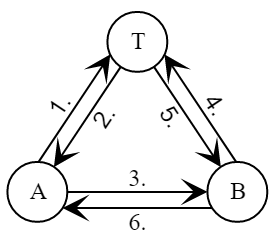
\includegraphics[width=0.5\textwidth]{pic/key_distribution-dass}
    \caption{Взаимодействие участников в протоколе DASS\label{fig:key_distribution-dass}}
\end{figure}

\begin{protocol}
    \item[(1)] $Alice \to \left\{ B \right\} \to Trent$
    \item[(2)] $Trent \to \left\{ S_T \left( B, K_B \right) \right\} \to Alice$
    \item[(3)] $Alice \to \left\{ E_K \left( T_A \right), S_A \left( L, A, K_P \right), S_{K_P} \left( E_B \left( K \right) \right) \right\} \to Bob$
    \item[(4)] $Bob \to \left\{ A \right\} \to Trent$
    \item[(5)] $Trent \to \left\{ S_T \left( A, K_A \right) \right\} \to Bob$
    \item[(6)] $Bob \to \left\{ E_K \left\{ T_B \right\} \right\} \to Alice$
\end{protocol}

С помощью сертификатов открытых ключей $\left\{ S_T \left( B, K_B \right) \right\}$ и $\left\{ S_T \left( A, K_A \right) \right\}$, которые отправляет Трент, и дальнейшего подтверждения владения соответствующими ключами, участники могут аутентифицировать друг-друга. Успешная расшифровка временных меток из сообщений $E_K \left( T_A \right)$ и $E_K \left\{ T_B \right\}$ обеспечивает подтверждение владением сеансовым ключом.

В протоколе используется время жизни ($L$) сеансового ключа $K_P$, однако в сообщение не включена метка времени. В результате протокол остаётся уязвимым к атаке с известным сеансовым ключом (KN)\index{атака!с известным сеансовым ключом}. Предположим, что Меллори смогла записать полностью прошедший сеанс связи между Алисой и Бобом, а потом смогла получить доступ к сеансовому ключу $K$. Это позволяет Меллори аутентифицировать себя как Алиса перед Бобом.

\begin{protocol}
    \item[(1)] $Mellory~(Alice) \to \left\{ E_K \left( T_M \right), S_A \left( L, A, K_P \right), S_{K_P} \left( E_B \left( K \right) \right) \right\} \to Bob$
    \item[(2)] $Bob \to \left\{ A \right\} \to Trent$
    \item[(3)] $Trent \to \left\{ S_T \left( A, K_A \right) \right\} \to Bob$
    \item[(4)] $Bob \to \left\{ E_K \left\{ T_B \right\} \right\} \to Mellory~(Alice)$
\end{protocol}

На первом проходе Меллори меняет только первое сообщение, содержащее метку времени $E_K \left( T_M \right)$. Всё остальное Меллори копирует из записанного сеанса связи. Если Боб не записывает используемые ключи, он не заметит подмены. Простейшее исправление данной уязвимости состоит во включении метки времени в сообщение $S_A \left( T_A, L, A, K_P \right)$.

Так как в протоколе сеансовый ключ $K$ шифруется <<мастер>>-ключом Боба $K_B$, то компрометация последнего приведёт к компрометации всех использованных ранее сеансовых ключей. То есть протокол не обеспечивает совершенной прямой секретности (цель G9).

Ни Трент, ни Боб не участвуют в формировании новых сеансовых ключей. Поэтому Алиса может заставить Боба использовать старый сеансовый ключ, как в протоколах Wide-Mouth Frog\index{протокол!Wide-Mouth Frog} (раздел~\ref{section-protocols-wide-moth-frog}) и Yahalom\index{протокол!Yahalom} (раздел~\ref{section-protocols-yahalom}).

\index{протокол!DASS|)}